\documentclass[aspectratio=169,12pt]{beamer}
\usepackage{amsmath}
\usepackage{amssymb}
\usepackage[most]{tcolorbox}
\usepackage{tikz}
\usepackage{graphicx}
\usepackage[sfdefault,lf]{FiraSans}
\renewcommand{\familydefault}{\sfdefault}
\setlength{\parindent}{0pt}
\everymath{\displaystyle}

\setbeamertemplate{navigation symbols}{}
\setbeamertemplate{footline}{}
\setbeamertemplate{headline}{}

\definecolor{mmpageWhite}{HTML}{FCFBF7}
\definecolor{mmtanSoft}{HTML}{F7F5EF}
\definecolor{mmgreenDeep}{HTML}{244B2C}
\definecolor{mmgreenLeaf}{HTML}{5D8A56}
\definecolor{mmgreenSoft}{HTML}{E4EFD9}
\definecolor{mmtext}{HTML}{163221}

\setbeamercolor{background canvas}{bg=mmpageWhite}
\setbeamercolor{normal text}{fg=mmtext,bg=mmpageWhite}

\newtcolorbox{MMProblemCard}[1][]{enhanced,breakable=false,colback=white,colframe=black,boxrule=1.5pt,arc=8pt,left=5pt,right=5pt,top=4pt,bottom=4pt,before skip=0pt,after skip=0pt,height=0.245\textheight,valign=top,#1}
\newcommand{\KoruIcon}{\raisebox{-0.2em}{
\includegraphics[height=1.05em]{../../SITE/header-logo.png}}}
\newcommand{\HoeIcon}{\raisebox{-0.2em}{
\includegraphics[height=1.05em]{../../SITE/hoe.png}}}
\newcommand{\ScaffoldIcons}[1]{\ifcase#1\or \HoeIcon\or \HoeIcon\hspace{0.22em}\KoruIcon\or \KoruIcon\hspace{0.22em}\KoruIcon\hspace{0.22em}\KoruIcon\fi}
\newcommand{\WorksheetTitle}[2]{%
  {\colorbox{mmtanSoft}{\parbox[c][2.0em][c]{0.975\linewidth}{%
    \hspace{0.25em}{\Large\bfseries\textcolor{mmgreenDeep}{#1}\hfill\ScaffoldIcons{#2}}}}
  \par\vspace{0.08em}{\color{mmgreenLeaf}\rule{\linewidth}{2.0pt}}\par\vspace{0.04em}}
}
\newcommand{\MMProblem}[2]{\begin{MMProblemCard}\raggedright\small\textbf{#1.} #2\par\end{MMProblemCard}}

\setbeamertemplate{background}{
 \begin{tikzpicture}[remember picture,overlay]
 \draw[black,line width=1.5pt,rounded corners=10pt]
 ([xshift=0.45cm,yshift=-0.45cm]current page.north west)
 rectangle
 ([xshift=-0.45cm,yshift=0.45cm]current page.south east);
 \end{tikzpicture}
}

% Default worksheet generation rules:
% use notes-style beamer pages
% use bordered cards for individual problems
% target 9 problems per frame in a 3x3 grid
% target 3 frames per scaffold by default where content allows

\begin{document}\begin{frame}[t]
\WorksheetTitle{Build Tasks}
\vspace{-0.18em}
\begin{columns}[T,onlytextwidth]
\begin{column}{0.32\textwidth}\MMProblem{1}{Name the marked angle in two different ways.\\[0.4em]
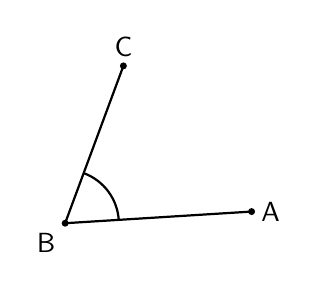
\begin{tikzpicture}[scale=0.74,baseline=(current bounding box.center)]
  \coordinate (B) at (0,0); \coordinate (A) at (3.2,0.2); \coordinate (C) at (1.0,2.7);
  \draw[thick] (B)--(A); \draw[thick] (B)--(C);
  \draw[thick] (0.92,0.06) arc[start angle=4,end angle=70,radius=0.92];
  \fill (A) circle (1.7pt) node[right] {A}; \fill (B) circle (1.7pt) node[below left] {B}; \fill (C) circle (1.7pt) node[above] {C};
\end{tikzpicture}}\end{column}
\begin{column}{0.32\textwidth}\MMProblem{2}{Name the marked angle in two different ways.\\[0.4em]
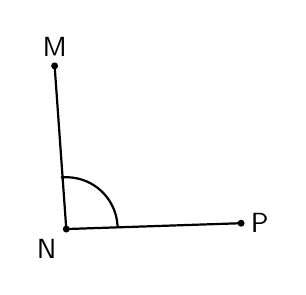
\begin{tikzpicture}[scale=0.74,baseline=(current bounding box.center)]
  \coordinate (N) at (0,0); \coordinate (M) at (-0.2,2.8); \coordinate (P) at (3.0,0.1);
  \draw[thick] (N)--(M); \draw[thick] (N)--(P);
  \draw[thick] (0.88,0.04) arc[start angle=2,end angle=96,radius=0.88];
  \fill (M) circle (1.7pt) node[above] {M}; \fill (N) circle (1.7pt) node[below left] {N}; \fill (P) circle (1.7pt) node[right] {P};
\end{tikzpicture}}\end{column}
\begin{column}{0.32\textwidth}\MMProblem{3}{The rays \mbox{$QX$} and \mbox{$QY$} form an angle. Write two correct names for it.}\end{column}
\end{columns}
\vspace{0.45em}
\begin{columns}[T,onlytextwidth]
\begin{column}{0.32\textwidth}\MMProblem{4}{The rays \mbox{$TS$} and \mbox{$TU$} form an angle. Write two correct names for it.}\end{column}
\begin{column}{0.32\textwidth}\MMProblem{5}{Which one is not a correct name for the same angle?\\[0.3em]\mbox{$\angle ABC$}, \mbox{$\angle CBA$}, \mbox{$\angle BAC$}}\end{column}
\begin{column}{0.32\textwidth}\MMProblem{6}{Which one is not a correct name for the same angle?\\[0.3em]\mbox{$\angle DEF$}, \mbox{$\angle FED$}, \mbox{$\angle DFE$}}\end{column}
\end{columns}
\vspace{0.45em}
\begin{columns}[T,onlytextwidth]
\begin{column}{0.32\textwidth}\MMProblem{7}{Write the vertex of each angle: \mbox{$\angle JKL$}, \mbox{$\angle PQR$}, \mbox{$\angle STU$}.}\end{column}
\begin{column}{0.32\textwidth}\MMProblem{8}{Copy and fix the wrong name. The angle has vertex \mbox{$B$} and arms through \mbox{$A$} and \mbox{$C$}, but it was written as \mbox{$\angle ACB$}.}\end{column}
\begin{column}{0.32\textwidth}\MMProblem{9}{Copy and fix the wrong name. The angle has vertex \mbox{$M$} and arms through \mbox{$L$} and \mbox{$N$}, but it was written as \mbox{$\angle LNM$}.}\end{column}
\end{columns}
\end{frame}
\begin{frame}[t]
\WorksheetTitle{Build Tasks}
\vspace{-0.18em}
\begin{columns}[T,onlytextwidth]
\begin{column}{0.32\textwidth}\MMProblem{1}{At one point, three rays \mbox{$OA$}, \mbox{$OB$} and \mbox{$OC$} are drawn. Name the small angle between \mbox{$OA$} and \mbox{$OB$}.}\end{column}
\begin{column}{0.32\textwidth}\MMProblem{2}{At one point, three rays \mbox{$RV$}, \mbox{$RW$} and \mbox{$RX$} are drawn. Name the angle between \mbox{$RW$} and \mbox{$RX$}.}\end{column}
\begin{column}{0.32\textwidth}\MMProblem{3}{Explain why \mbox{$\angle ABC$} and \mbox{$\angle CBA$} can name the same angle, but \mbox{$\angle BAC$} cannot.}\end{column}
\end{columns}
\vspace{0.45em}
\begin{columns}[T,onlytextwidth]
\begin{column}{0.32\textwidth}\MMProblem{4}{}\end{column}
\begin{column}{0.32\textwidth}\MMProblem{5}{}\end{column}
\begin{column}{0.32\textwidth}\MMProblem{6}{}\end{column}
\end{columns}
\vspace{0.45em}
\begin{columns}[T,onlytextwidth]
\begin{column}{0.32\textwidth}\MMProblem{7}{}\end{column}
\begin{column}{0.32\textwidth}\MMProblem{8}{}\end{column}
\begin{column}{0.32\textwidth}\MMProblem{9}{}\end{column}
\end{columns}
\end{frame}
\end{document}
